\documentclass[11pt]{article}

\usepackage[utf8]{inputenc}
\usepackage[T1]{fontenc}
\usepackage{lmodern}
\usepackage[margin=1in]{geometry}
\usepackage{microtype}
\emergencystretch=3em
\usepackage{amsmath,amssymb,amsthm,mathtools}
\usepackage{bbm}
\usepackage{booktabs}
\usepackage{longtable}
\usepackage{array}
\usepackage[table]{xcolor}
\usepackage{enumitem}
\usepackage{tikz}
\usetikzlibrary{arrows.meta,positioning,calc,fit}
\usepackage[hidelinks]{hyperref}
\usepackage[nameinlink,noabbrev]{cleveref}
\usepackage{authblk}

\setlist[itemize]{leftmargin=1.5em}
\setlist[enumerate]{leftmargin=1.5em}
\renewcommand{\arraystretch}{1.15}
\setlength{\extrarowheight}{1pt}
\setlength{\LTpre}{0.6em}
\setlength{\LTpost}{0.6em}

\newtheorem{definition}{Definition}[section]
\newtheorem{axiom}{Axiom}[section]
\newtheorem{proposition}{Proposition}[section]
\newtheorem{conjecture}{Conjecture}[section]
\newtheorem{remark}{Remark}[section]
\newtheorem{example}{Example}[section]

\newcommand{\Phys}{\mathbf{Phys}}
\newcommand{\Math}{\mathbf{Math}}
\newcommand{\Dom}{\mathbf{Dom}}
\newcommand{\Rep}{\mathbf{Rep}}
\newcommand{\Obs}{\mathbf{Obs}}
\newcommand{\Real}{\operatorname{Real}}
\newcommand{\Mot}{\operatorname{Mot}}
\newcommand{\Aut}{\operatorname{Aut}}
\newcommand{\Spec}{\operatorname{Spec}}
\newcommand{\Bord}{\operatorname{Bord}}
\newcommand{\Vect}{\operatorname{Vect}}
\newcommand{\Hilb}{\operatorname{Hilb}}
\newcommand{\End}{\operatorname{End}}
\newcommand{\per}{\operatorname{per}}
\newcommand{\id}{\operatorname{id}}
\newcommand{\op}{\mathrm{op}}
\newcommand{\Sstd}{\textsf{S}}
\newcommand{\Sheur}{\textsf{H}}
\newcommand{\Pspec}{\textsf{P}}
\newcommand{\status}[1]{\textsf{#1}}
\newcommand{\entry}[4]{#1 & #2 & #3 & \status{#4}\\}
\newcommand{\physbracket}[1]{[\![ #1 ]\!]_{\mathrm{phys}}}

\title{A Representation-Stack Library for Mathematical Structures in Physical Representation\\
\large Motives, Periods, Coalgebras, Gauge Redundancy, and Quantum-Informational Availability}

\author[1]{Anonymous Draft}
\affil[1]{Conceptual mathematics and mathematical physics research note}
\date{\today}

\begin{document}
\maketitle

\begin{abstract}
We propose a formal framework for a mathematics-to-physics representation library. The organizing thesis is that many physical quantities are not merely described by mathematics, but are obtained as realizations of structured mathematical information. The framework is expressed as a representation stack: abstract mathematical structures are interpreted through realization functors into physical representations and then into observables. The paper organizes algebraic geometry, algebraic topology, category theory, homotopy type theory, sheaf and stack theory, motivic periods, Lie coalgebras, Hopf algebras, and quantum-information error-protection into a single status-labeled dictionary. Standard correspondences, such as topological quantum field theories as functors from cobordism categories, categorical quantum mechanics via dagger-compact categories, gauge fields as local data with descent, and Feynman amplitudes as period-like integrals, are separated from heuristic and speculative ontological extensions. A central guiding formula is
\[
\text{observable}=\Real(\text{abstract structure}),
\]
while the motivic refinement reads
\[
\mathcal A = \per(\mathcal A^{\mathfrak m}),\qquad
\Delta(\mathcal A^{\mathfrak m})=\sum_i \mathcal A^{\mathfrak m}_{i,1}\otimes \mathcal A^{\mathfrak m}_{i,2}.
\]
This formalizes the claim that coalgebraic and motivic structures can encode how physical amplitudes, periods, and observables decompose into primitive informational pieces. The result is not presented as an established physical theory, but as an extensible research language for comparing representation, realization, measurement, symmetry redundancy, and logical information across several mature mathematical frameworks.
\end{abstract}

\noindent\textbf{Keywords:} motives; periods; physical representation; stacks; gauge redundancy; algebraic topology; algebraic geometry; HoTT; category theory; Lie coalgebras; Hopf algebras; quantum information.

\tableofcontents

\section{Introduction}

Mathematical physics contains many precise examples in which a physical theory is naturally expressed as a translation from one mathematical category to another. Atiyah's axioms for topological quantum field theory place an $n$-dimensional TQFT in the form of a symmetric monoidal functor from a bordism category to vector spaces \cite{Atiyah1988}. Lurie's formulation of the cobordism hypothesis refines this idea to extended field theories and higher categories \cite{Lurie2009}. Categorical quantum mechanics expresses quantum protocols using compact closed and dagger-compact categorical structures \cite{AbramskyCoecke2004,BaezStay2009}. Homotopy type theory interprets identity types as path-like structures and univalence as the principle that equivalent types may be identified \cite{HoTT2013}. Feynman amplitudes are often periods or period-like integrals and are connected with algebraic geometry, motives, multiple polylogarithms, and Hopf-algebraic renormalization \cite{KontsevichZagier2001,ConnesKreimer1999,Goncharov2001,Brown2015Periods,BlochEsnaultKreimer2006}.

The present paper assembles these examples into a single representation library. The guiding phrase is:
\[
\boxed{\begin{minipage}{0.87\textwidth}\centering
algebraic structure encoding how physical amplitudes, periods, and observables\
decompose into primitive informational pieces
\end{minipage}}
\]
We interpret this phrase as a program for organizing mathematical structures by the physical roles they play: composition, decomposition, localization, gauge equivalence, realization, measurement, and informational robustness.

The key move is to distinguish three levels:
\[
\textbf{abstract structure}\longrightarrow \textbf{realization}\longrightarrow \textbf{physical representation}\longrightarrow \textbf{observable/measurement}.
\]
This is not meant to erase the distinction between mathematics and physics. Rather, it is a language for tracking when a mathematical structure is used as a rigorous model, when it is used as a heuristic analogy, and when it is used as a speculative ontological proposal.

\subsection{Contributions}

The paper contributes the following conceptual formalization.
\begin{enumerate}
    \item A \emph{representation-stack} formalism: local mathematical-physical translations form a prestack over domains of mathematics, and become stack-like when compatible local interpretations glue up to equivalence.
    \item A status system distinguishing standard mathematical-physics correspondences (\Sstd), strong heuristic dictionary entries (\Sheur), and speculative ontological extensions (\Pspec).
    \item A motivic interpretation of ``the functions of'' an object: not as a replacement for the standard definition of motives, but as a semantic layer in which motives serve as pre-numerical functional cores behind realizations.
    \item A coalgebraic anatomy of amplitudes: motivic or period-like amplitudes admit coproduct/coaction/cobracket operations that decompose observables into lower-complexity informational pieces.
    \item A stack-theoretic account of gauge redundancy and a quantum-information interpretation of high availability: many local or physical representatives can encode the same logical or physical content.
\end{enumerate}

\subsection{Epistemic status}

We use the following status labels throughout.
\begin{center}
\begin{tabular}{@{}lll@{}}
\toprule
Label & Meaning & Example \\
\midrule
\Sstd & standard use in mathematics or mathematical physics & TQFT as a functor $\Bord_n\to\Vect$ \\
\Sheur & strong heuristic representation dictionary & motive as functional essence \\
\Pspec & speculative philosophical ontology & physical reality as motivic-categorical realization \\
\bottomrule
\end{tabular}
\end{center}
This separation is crucial. The framework proposed here is intended to be useful precisely because it does not present every analogy as an established theorem.

\section{From dictionary to representation stack}

\subsection{Basic notation}

Let $\Dom$ be a category whose objects are mathematical domains, such as algebraic topology, algebraic geometry, category theory, homotopy type theory, sheaf/stack theory, and motivic period theory. Let each $d\in\Dom$ have an associated category or higher category $\Math_d$ of mathematical structures in that domain. Let $\Phys$ denote a category, bicategory, or $\infty$-category of physical representation targets: state spaces, observable algebras, process categories, gauge moduli stacks, quantum code spaces, or measurement outcomes.

The notation
\[
\physbracket{M}
\]
denotes the physical representation assigned to a mathematical structure $M$ when a chosen interpretation is understood.

\begin{definition}[Representation entry]
A \emph{representation entry} is a quadruple
\[
E=(M,P,\tau,\sigma),
\]
where $M\in\Math_d$ is a mathematical structure, $P\in\Phys$ is a proposed physical representation, $\tau$ is a semantic translation datum, and
\[
\sigma\in\{\Sstd,\Sheur,\Pspec\}
\]
is an epistemic status label.
\end{definition}

The semantic translation datum $\tau$ may be an actual functor, a natural transformation, an equivalence class of models, a physical interpretation map, or a weaker relation. For example, in standard TQFT the translation datum is a symmetric monoidal functor. In a heuristic dictionary entry, it may be an interpretation rule such as ``cohomology class $\mapsto$ stable observable.''

\begin{definition}[Representation library]
A \emph{mathematics-to-physics representation library} is a collection of representation entries closed under the following operations when these operations are defined:
\begin{enumerate}
    \item restriction to subdomains,
    \item transport along equivalence of mathematical structures,
    \item composition of compatible translations,
    \item decomposition through boundary, coproduct, or localization operations,
    \item realization into observables.
\end{enumerate}
\end{definition}

\subsection{The representation stack}

The library becomes stack-like when local entries glue, not necessarily by equality, but by equivalence. This captures the phenomenon that local descriptions of a physical system often agree only up to gauge transformation.

\begin{definition}[Representation prestack]
A \emph{representation prestack} is a pseudofunctor
\[
\Rep_{\mathrm{phys}}:\Dom^{\op}\longrightarrow \mathbf{Gpd},
\]
assigning to each domain $d$ a groupoid of representation entries in that domain, and assigning to a domain inclusion or refinement $u:e\to d$ a restriction functor
\[
u^\ast:\Rep_{\mathrm{phys}}(d)\to \Rep_{\mathrm{phys}}(e).
\]
\end{definition}

\begin{definition}[Representation stack]
Let $\Dom$ be equipped with a Grothendieck topology expressing domain coverage or local contextual coverage. A representation prestack $\Rep_{\mathrm{phys}}$ is a \emph{representation stack} if compatible families of local representation entries glue to global entries, and if the gluing is unique up to a coherent isomorphism.
\end{definition}

\begin{remark}
The word ``stack'' is used here in a formal but deliberately broad sense. In ordinary geometry, stacks encode descent with automorphisms. Here, the automorphisms represent gauge changes, duality transformations, code stabilizers, or other equivalences that do not change the relevant physical content.
\end{remark}

\subsection{The realization pipeline}

The universal representation pipeline is
\[
M\in\Math_d
\xrightarrow{\Phi}
\text{abstract physical-information object}
\xrightarrow{\Real_\alpha}
\text{physical representation}
\xrightarrow{\Obs}
\text{measurement data}.
\]
Equivalently,
\[
\boxed{\Obs_\alpha(M)=\Obs\bigl(\Real_\alpha(\Phi(M))\bigr).}
\]
The index $\alpha$ labels the realization channel: Betti, de Rham, Hodge, etale, $p$-adic, quantum, thermodynamic, computational, experimental, or operational.

\begin{axiom}[Realization]
A physical observable is represented as the output of a realization channel applied to an abstract structure:
\[
\text{observable}=\Obs\circ\Real_\alpha(\text{abstract structure}).
\]
\end{axiom}

\begin{axiom}[Equivalence]
If two mathematical descriptions are related by an equivalence that lies in the automorphism or gauge groupoid of a representation entry, then they determine the same physical content at the chosen level of observation.
\end{axiom}

\begin{axiom}[Locality/descent]
Physical representations must be locally assignable and globally coherent. Failure of descent is interpreted as an obstruction, anomaly, or missing boundary datum.
\end{axiom}

\begin{axiom}[Decomposition]
For compositional or period-like observables, there exists a decomposition operation, such as a boundary, coproduct, coaction, spectral sequence, or factorization rule, that reveals lower-level informational pieces.
\end{axiom}

\subsection{A master diagram}

\begin{center}
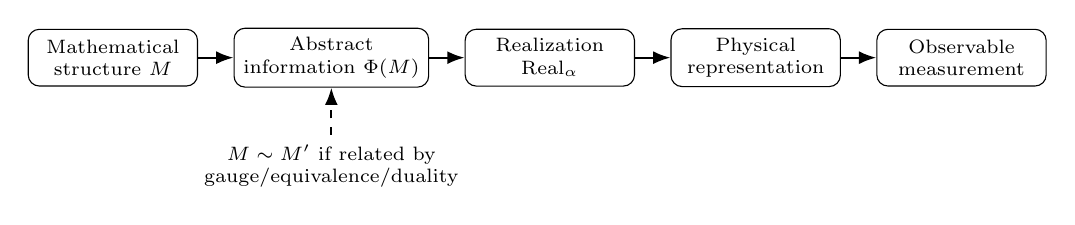
\begin{tikzpicture}[node distance=0.45cm and 0.45cm, every node/.style={font=\scriptsize}, box/.style={draw, rounded corners, align=center, minimum width=2.15cm, minimum height=0.72cm}, arr/.style={-{Latex[length=2.2mm]}, thick}]
\node[box] (M) {Mathematical\\structure $M$};
\node[box, right=of M] (Phi) {Abstract\\information $\Phi(M)$};
\node[box, right=of Phi] (R) {Realization\\$\Real_\alpha$};
\node[box, right=of R] (P) {Physical\\representation};
\node[box, right=of P] (O) {Observable\\measurement};
\draw[arr] (M) -- (Phi);
\draw[arr] (Phi) -- (R);
\draw[arr] (R) -- (P);
\draw[arr] (P) -- (O);
\node[below=0.6cm of Phi, align=center] (eq) {$M\sim M'$ if related by\\gauge/equivalence/duality};
\draw[arr, dashed] (eq) -- (Phi);
\end{tikzpicture}
\end{center}

\section{Motives as functional essence}

The word ``motive'' has a precise mathematical history. In Grothendieck's vision, motives should function as universal objects behind cohomology theories. A variety $X$ has several cohomological realizations, and the motive $\Mot(X)$ is a universal source from which these realizations are extracted. This standard picture may be summarized by
\[
H_\alpha(X)\simeq \Real_\alpha(\Mot(X)),
\]
where $\alpha$ may denote Betti, de Rham, Hodge, etale, or another realization.

The semantic proposal of this paper is not to redefine motives, but to add a representational reading:
\[
\boxed{\Mot(X)=\text{the invariant functional essence of }X.}
\]
In the language proposed by the user motivating this manuscript, a motive is the representational structure encoding ``the functions of'' a thing. More precisely, it is the invariant pre-numerical source from which different functional readings of the object can be obtained.

\begin{definition}[Functional-essence interpretation]
A \emph{functional-essence interpretation} is a status-\Sheur{} semantic rule
\[
\mathsf{FE}(X):=\Mot(X),
\]
read as ``the invariant structure from which the functions, cohomological readings, periods, and numerical shadows of $X$ are realized.''
\end{definition}

This yields the chain
\[
\boxed{
X\longmapsto \Mot(X)\longmapsto \Real_\alpha(\Mot(X))\longmapsto \text{physical observable}.
}
\]
It is often useful to distinguish the motivic level from the numerical level. Let $\mathcal A^{\mathfrak m}$ be a motivic amplitude object and $\per$ a period map. Then
\[
\boxed{\mathcal A=\per(\mathcal A^{\mathfrak m})}
\]
expresses a physical amplitude as a numerical realization of pre-numerical motivic data.

\section{Periods, amplitudes, and coalgebraic anatomy}

\subsection{Period data}

Kontsevich and Zagier describe periods as numbers given by integrals of algebraic differential forms over domains specified by algebraic equations or inequalities \cite{KontsevichZagier2001}. In physical language, a period is a numerical shadow of a geometric pairing:
\[
\int_\Gamma \omega.
\]
Here $\omega$ is a differential form and $\Gamma$ is an integration cycle or relative chain.

\begin{definition}[Period datum]
A \emph{period datum} is a tuple
\[
\Pi=(X,D,\omega,\Gamma),
\]
where $X$ is an algebraic or analytic space, $D$ is boundary or divisor data, $\omega$ is a differential form on $X\setminus D$, and $\Gamma$ is a cycle or relative chain. Its numerical period is
\[
\per(\Pi)=\int_\Gamma \omega.
\]
\end{definition}

A Feynman integral can often be placed into this pattern after choosing an appropriate representation, regularization, or compactification. Bloch, Esnault, and Kreimer studied motives associated to graph polynomials, motivated by the appearance of multiple zeta values in renormalization data \cite{BlochEsnaultKreimer2006}. Brown reviewed the role of periods and motivic periods in Feynman amplitudes \cite{Brown2015Periods,Brown2015Cosmic}. Goncharov developed multiple polylogarithms from analytic, Hodge, and motivic perspectives and described Hopf-algebraic structures on them \cite{Goncharov2001}.

\subsection{Amplitude objects}

\begin{definition}[Motivic amplitude object]
A \emph{motivic amplitude object} is a pre-numerical object $\mathcal A^{\mathfrak m}$ in a category or comodule of motivic periods whose numerical realization is a physical amplitude:
\[
\per(\mathcal A^{\mathfrak m})=\mathcal A.
\]
\end{definition}

The central decomposition principle is that $\mathcal A^{\mathfrak m}$ may admit a coproduct or coaction
\[
\Delta(\mathcal A^{\mathfrak m})=\sum_i \mathcal A^{\mathfrak m}_{i,1}\otimes \mathcal A^{\mathfrak m}_{i,2}.
\]
This should be interpreted as a full hierarchical anatomy map. A cobracket
\[
\delta:\mathcal L\longrightarrow \Lambda^2\mathcal L
\]
extracts a primitive antisymmetric part of the decomposition.

\begin{definition}[Coalgebraic anatomy]
Given a class of observable objects $\mathcal O$ equipped with a coalgebraic operation $\Delta$ or $\delta$, the \emph{coalgebraic anatomy} of an observable $O\in\mathcal O$ is the system of lower-complexity pieces obtained by iterating the decomposition operations.
\end{definition}

\begin{proposition}[Conditional amplitude decomposition]
Suppose motivic amplitude objects form a comodule over a Hopf algebra of motivic periods. Then the coaction defines a representation-stable decomposition of amplitudes into tensorial pieces, and every compatible realization channel transports this decomposition to the corresponding analytic or numerical amplitude representation.
\end{proposition}

\begin{proof}
This is a formal property of comodules and functorial realization. If $\Delta$ is the comodule structure and $\Real_\alpha$ is compatible with the relevant tensor product, then applying $\Real_\alpha$ to the coaction identity gives a corresponding decomposition in the target category. The physical content of the statement depends on whether the amplitudes under consideration actually admit such motivic lifts and compatible realizations.
\end{proof}

\subsection{Coproducts, cuts, and factorization}

The dictionary proposed here reads:
\[
\Delta=\text{full anatomy map},\qquad
\delta=\text{primitive information split}.
\]
In amplitude language, such decompositions may be compared with cuts, factorization channels, branch discontinuities, residues, and boundary strata of positive geometries. Positive geometries and canonical forms provide one rigorous setting in which boundaries and residues are linked to scattering-amplitude structures \cite{ArkaniHamedBaiLam2017}.

\section{Algebraic geometry: spaces of physical possibility}

Algebraic geometry contributes the language of solution spaces, moduli, singularities, compactifications, sheaves, stacks, periods, and arithmetic refinements. The core representation principle is
\[
\boxed{\text{algebraic geometry}=\text{geometry of physical possibilities}.}
\]
A coordinate ring is an algebra of functions; physically, this suggests that observables generate the space. A quotient ring $R/I$ represents functions modulo constraints, which can be read as the on-shell observable algebra. A moduli stack retains automorphisms and therefore models gauge-correct configuration spaces.

\begin{example}[On-shell observable algebra]
Let $R$ be an algebra of fields or coordinates and $I$ the ideal generated by equations of motion or constraints. Then $R/I$ is a natural algebraic representation of observables modulo the imposed physical equations. This entry is standard in algebraic approaches to field theory, but its ontological reading as ``measurements generate space'' is heuristic.
\end{example}

\begin{example}[Positive geometry]
A positive geometry is a geometric region equipped with a canonical form whose boundary residues recursively encode lower-dimensional canonical forms. In scattering-amplitude applications, this gives a precise model of how geometric boundaries can represent physical singularities or factorization channels \cite{ArkaniHamedBaiLam2017}.
\end{example}

\section{Algebraic topology: conserved global information}

Algebraic topology contributes invariants that survive continuous deformation: homotopy classes, homology, cohomology, characteristic classes, generalized cohomology, K-theory, and bordism. The core representation principle is
\[
\boxed{\text{algebraic topology}=\text{grammar of conserved global information}.}
\]
A cohomology class is a stable observable insensitive to local deformation. Characteristic classes encode quantized topological information in bundles. Spin structures control the possibility of globally defining fermions. Bordism groups and generalized cohomology theories classify topological phases and anomalies in many modern settings. Dijkgraaf-Witten theory gives a concrete example in which group cohomology defines topological gauge theories for finite groups \cite{DijkgraafWitten1990}.

\section{Category theory and HoTT: composition and identity}

Category theory turns attention from objects to morphisms, composition, functorial translation, and universal properties. The representation principle is
\[
\boxed{\text{category theory}=\text{grammar of physical composition}.}
\]
A physical theory may be a functor, a duality may be an equivalence of categories, and a process may be a morphism. In TQFT, the functorial slogan is
\[
Z:\Bord_n\longrightarrow \mathcal C,
\]
where boundaries are assigned state objects and cobordisms are assigned processes \cite{Atiyah1988,Lurie2009}.

Homotopy type theory contributes an internal logic of spaces, paths, equivalences, and higher identities. The representation principle is
\[
\boxed{\text{HoTT}=\text{logic of spaces, paths, equivalences, and higher identity}.}
\]
A type $A$ may be read as a space of possibilities, a term $a:A$ as an actual state or witness, an identity type $a=b$ as a path or equivalence, and a dependent type $B(x)$ as a field of data over a base configuration. The univalence principle supports the representation-theoretic slogan
\[
\boxed{\text{equivalent representations can be treated as the same physical content}.}
\]
Cohesive and differential refinements of higher topos theory and type theory further connect these ideas with gauge fields, differential cohomology, Chern-Weil theory, and higher geometric structures \cite{Schreiber2013}.

\section{Sheaves, stacks, gauge redundancy, and quantum high availability}

\subsection{Symmetry redundancy}

Symmetry redundancy means that different mathematical descriptions represent the same physical state. Gauge theory is the archetypal example. In electromagnetism, the gauge potential $A$ may change by
\[
A\mapsto A+d\lambda,
\]
while the field strength
\[
F=dA
\]
is unchanged because $d^2=0$. The physical state is not the raw potential; it is the equivalence class of potentials modulo gauge transformation, together with possible global and automorphism data.

\begin{definition}[Gauge redundancy]
Let $X$ be a space of mathematical descriptions and $G$ a group or groupoid acting on $X$. A \emph{gauge redundancy} is an action for which points in the same orbit represent the same physical content at the chosen observational level.
\end{definition}

The coarse quotient $X/G$ identifies equivalent descriptions, but the quotient stack $[X/G]$ retains stabilizers:
\[
\Aut_{[X/G]}(x)\simeq \operatorname{Stab}_G(x).
\]
Thus a stack is not merely a quotient; it remembers how descriptions are equivalent.

\begin{proposition}[Stacks retain gauge information]
If a physical configuration space is represented by descriptions $X$ modulo gauge transformations $G$, and if stabilizer groups influence observables, anomalies, quantization, or path-integral weights, then the quotient stack $[X/G]$ is a more faithful representation object than the coarse quotient $X/G$.
\end{proposition}

\begin{proof}
The coarse quotient records orbits but generally forgets automorphism groups of representatives. The stack quotient records objects, equivalences, and self-equivalences. Gauge-theoretic data such as residual symmetry, isotropy, and automorphism factors live in these self-equivalences, so retaining the stack structure preserves information discarded by the coarse quotient.
\end{proof}

\subsection{Quantum-information high availability}

In classical high availability, information is often protected by replication. In quantum information, arbitrary quantum states cannot simply be copied; robust storage is achieved by encoding logical information into a larger physical Hilbert space. Topological codes and anyonic models are standard examples of fault-tolerant encodings in which information is protected by global or topological structure \cite{Kitaev1997}.

The representation-stack viewpoint suggests the following dictionary:
\[
\boxed{\text{many physical representatives}\longrightarrow \text{one logical/observable content}.}
\]
A stabilizer quantum code has operators $s$ satisfying
\[
 s|\psi_L\rangle=|\psi_L\rangle
\]
for logical code states $|\psi_L\rangle$. In a subsystem code, the physical Hilbert space may decompose schematically as
\[
\mathcal H_{\mathrm{phys}}\simeq \mathcal H_{\mathrm{logical}}\otimes \mathcal H_{\mathrm{gauge}}\oplus \mathcal H_{\mathrm{error}},
\]
where changes in the gauge subsystem do not change the encoded logical content. This is the quantum-information cousin of gauge redundancy.

\begin{definition}[Quantum high-availability representation]
A \emph{quantum high-availability representation} is an encoding
\[
\iota:\mathcal H_{\mathrm{logical}}\hookrightarrow \mathcal H_{\mathrm{phys}}
\]
together with an equivalence groupoid of physical variations such that logical observables are invariant under the allowed variations and detectable/correctable errors move the system within controlled equivalence or syndrome sectors.
\end{definition}

\begin{remark}
The analogy with stacks is structural: a sheaf stores compatible local data; a stack stores compatible local data plus automorphisms; a quantum code stores logical data across physical degrees of freedom plus transformations that do not change the logical content. This is not a claim that every quantum code is literally a stack, but it suggests a useful representation language for fault tolerance, gauge subsystems, and topological order.
\end{remark}

\section{Axioms for a representation ontology}

The following axioms summarize the proposed research program.

\begin{axiom}[Syntax]
Mathematical structures supply the syntax of representation: objects, morphisms, spaces, paths, functions, forms, cycles, symmetries, and decompositions.
\end{axiom}

\begin{axiom}[Semantics]
A physical interpretation is a semantic assignment from mathematical structures to physical roles. This assignment must record its epistemic status: standard, heuristic, or speculative.
\end{axiom}

\begin{axiom}[Realization]
Measurements are obtained only after choosing a realization channel. Different realization channels can expose different physical readings of the same abstract structure.
\end{axiom}

\begin{axiom}[Equivalence/gauge]
Physical content is invariant under designated equivalences. The correct representation object should retain the automorphisms of these equivalences when they affect physical or informational behavior.
\end{axiom}

\begin{axiom}[Decomposition]
Composite observables should be studied through decomposition operations: boundary, residue, coproduct, coaction, spectral sequence, localization, or factorization.
\end{axiom}

\begin{axiom}[Motivic pre-numericality]
When physical observables are periods or period-like quantities, their numerical values should be distinguished from the pre-numerical structures whose realizations produce them.
\end{axiom}

\begin{conjecture}[Motivic-categorical information ontology]
A sufficiently broad class of physical theories admits a representation-stack description in which states, processes, observables, amplitudes, gauge redundancies, and measurement values arise as realizations of structured categorical, homotopical, geometric, and motivic information.
\end{conjecture}

The conjecture is intentionally broad. Its value lies in generating testable subprograms: identify the domain, define the representation entries, specify the realization channels, distinguish equivalences from physical transformations, and compute decomposition operations.

\section{Limitations and criteria for use}

The framework is not a replacement for physical modeling, experiment, or established mathematical definitions. Several cautions are necessary.

\begin{enumerate}
    \item Not every mathematical analogy is a physical theory. The status labels are part of the formalism.
    \item Motives are not literally defined as ``the functions of'' an object in standard mathematics; that phrase is a semantic interpretation proposed for this library.
    \item A single universal functor from all mathematics to all physics is unlikely to be well-defined. The representation-stack approach is deliberately local and domain-indexed.
    \item Some physical observables are not known to be periods, and some amplitudes require elliptic, modular, non-Tate, or more general analytic structures.
    \item Gauge redundancy is not the same as physical symmetry. Physical symmetries can map one physical state to another; gauge symmetries identify different descriptions of the same physical content.
\end{enumerate}

\section{Conclusion}

The proposed library can be compressed into four slogans:
\[
\boxed{\text{mathematics is the syntax of physical representation};}
\]
\[
\boxed{\text{motives are functional semantics};}
\]
\[
\boxed{\text{periods are numerical measurements};}
\]
\[
\boxed{\text{coalgebras are decomposition laws}.}
\]
More formally, a physical observable is modeled as a realization of an abstract mathematical object, and a decomposable observable is modeled by equipping that object with boundary, coproduct, coaction, or cobracket structure. Algebraic topology tracks conserved global information. Algebraic geometry tracks spaces of possibility and singularities. Category theory tracks composition and translation. HoTT tracks identity and equivalence. Sheaves and stacks track local-to-global information with gauge redundancy. Motives track pre-numerical functional essence. Periods track measured numerical shadows. Lie coalgebras and Hopf algebras track the anatomy of amplitudes, renormalization, and primitive informational pieces.

The resulting framework is not the final ontology of physics. It is a disciplined language for building one.

\appendix
\section{Core translation library}
\footnotesize
\rowcolors{2}{gray!6}{white}
\begin{longtable}{@{}>{\raggedright\arraybackslash}p{0.23\textwidth}>{\raggedright\arraybackslash}p{0.27\textwidth}>{\raggedright\arraybackslash}p{0.35\textwidth}>{\centering\arraybackslash}p{0.05\textwidth}@{}}
\toprule
Mathematics & Physical representation & Semantic interpretation & Status\\
\midrule
\endfirsthead
\toprule
Mathematics & Physical representation & Semantic interpretation & Status\\
\midrule
\endhead
\bottomrule
\endfoot
\entry{Mathematical object $X$}{Physical system or possible world-structure}{Structured carrier of physical information}{H}
\entry{Representation $\rho:X\to \End(V)$}{Physical realization on states}{How abstract structure acts on observables or states}{S}
\entry{Realization functor}{Translation into measurable form}{Passage from abstract information to physically readable data}{S/H}
\entry{Invariant}{Conservation law or observable quantity}{What remains stable under allowed transformations}{S}
\entry{Equivalence}{Same physics in different mathematical coordinates}{Dual descriptions, gauge equivalence, change of representation}{S}
\entry{Symmetry}{Redundancy or physical transformation}{Law preserving structure}{S}
\entry{Duality}{Two theories with same physical content}{Equivalence between representation languages}{S}
\entry{Moduli space}{Space of physically distinct configurations}{Parameter space of possible structures}{S}
\entry{Quotient}{Identification of redundant descriptions}{Gauge reduction or physical state space}{S}
\entry{Boundary}{Physical interface or asymptotic region}{Where factorization, measurement, or interaction appears}{S/H}
\entry{Singularity}{Threshold, phase transition, divergent region}{Breakdown or special physical regime}{S/H}
\entry{Decomposition}{Factorization, cut, measurement split}{Observable broken into primitive pieces}{S}
\entry{Primitive}{Irreducible informational unit}{Cannot be decomposed further inside the chosen grammar}{H}
\entry{Functor}{Physical theory as translation}{Assigns states to spaces and processes to histories}{S}
\entry{Natural transformation}{Equivalence or deformation of theories}{Consistent translation between physical descriptions}{S/H}
\entry{Category}{Universe of systems and processes}{Objects are systems; morphisms are allowed transitions}{S/H}
\end{longtable}

\section{Motivic and amplitude library}
\begin{longtable}{@{}>{\raggedright\arraybackslash}p{0.23\textwidth}>{\raggedright\arraybackslash}p{0.27\textwidth}>{\raggedright\arraybackslash}p{0.35\textwidth}>{\centering\arraybackslash}p{0.05\textwidth}@{}}
\toprule
Mathematics & Physical representation & Decomposition meaning & Status\\
\midrule
\endfirsthead
\toprule
Mathematics & Physical representation & Decomposition meaning & Status\\
\midrule
\endhead
\bottomrule
\endfoot
\entry{Field $F$}{Kinematic or coordinate domain}{Allowed values of physical parameters}{S/H}
\entry{$F^\times$}{Nonzero scales or ratios}{Energies, masses, cross-ratios, coupling ratios}{S/H}
\entry{Cross-ratio}{Conformal invariant}{Dimensionless observable independent of scale}{S}
\entry{Algebraic variety}{Constraint solution space}{Allowed configurations satisfying equations}{S}
\entry{Graph hypersurface}{Geometry associated to Feynman graph}{Algebraic container of graph integral data}{S}
\entry{Feynman integral}{Period integral}{Observable from pairing geometry and domain}{S}
\entry{Period}{Measurable number from geometry}{Numerical shadow of deeper structure}{S}
\entry{Period pairing $\int_\Gamma\omega$}{Observable amplitude contribution}{Pairing of form and integration cycle}{S}
\entry{Differential form $\omega$}{Integrand or local observable density}{What is being accumulated}{S}
\entry{Cycle $\Gamma$}{Integration domain, path, history class}{Where physical accumulation occurs}{S}
\entry{Relative cohomology}{Boundary-sensitive observable}{Observable with cuts, thresholds, or boundaries}{S}
\entry{Motive}{Pre-numerical functional essence}{Hidden source of periods}{S/H}
\entry{Mixed motive}{Layered informational object}{Amplitude with multiple weights and depths}{S/H}
\entry{Mixed Tate motive}{Polylogarithmic period structure}{Tame amplitude period class}{S}
\entry{Non-Tate motive}{More complex amplitude geometry}{Elliptic, Calabi-Yau, or modular sectors}{S}
\entry{Multiple zeta value}{Special period}{Constant term in loop or amplitude expansions}{S}
\entry{Polylogarithm $\operatorname{Li}_n(x)$}{Layered propagation function}{Iterated amplitude contribution}{S}
\entry{Multiple polylogarithm}{Multi-scale iterated propagation}{Nested channel dependence}{S}
\entry{Symbol of polylogarithm}{First-order function decomposition}{Branch-cut or discontinuity data}{S}
\entry{Coproduct/coaction}{Decomposition of period}{How amplitude splits into lower pieces}{S}
\entry{Cobracket $\delta$}{Antisymmetric primitive split}{Factorization channel or information split}{H}
\entry{Goncharov coproduct}{Motivic decomposition operation}{Arithmetic anatomy of polylogs}{S}
\entry{Goncharov Lie coalgebra}{Coalgebra of polylog motivic data}{Grammar of primitive amplitude data}{S/H}
\entry{Weight grading}{Transcendental complexity}{Loop depth or functional complexity}{S/H}
\entry{Depth grading}{Iterated-integral nesting}{Number of nested propagation layers}{S/H}
\entry{Primitive element}{Indecomposable motivic component}{Irreducible informational contribution}{H}
\entry{Regulator map}{Motive to analytic number}{Measurement or numerical extraction}{S/H}
\entry{Hodge realization}{Analytic-geometric reading}{Differential-form representation}{S}
\entry{de Rham realization}{Form/integrand side}{Calculational analytic representation}{S}
\entry{Betti realization}{Cycle/topological side}{Path or integration-domain representation}{S}
\entry{Etale realization}{Arithmetic/discrete realization}{Number-theoretic shadow}{S/H}
\entry{Cosmic Galois group}{Symmetry acting on periods}{Hidden symmetry organizing amplitudes}{H/P}
\end{longtable}

\section{Algebraic geometry library}
\begin{longtable}{@{}>{\raggedright\arraybackslash}p{0.23\textwidth}>{\raggedright\arraybackslash}p{0.27\textwidth}>{\raggedright\arraybackslash}p{0.35\textwidth}>{\centering\arraybackslash}p{0.05\textwidth}@{}}
\toprule
Algebraic geometry & Physical representation & Semantic meaning & Status\\
\midrule
\endfirsthead
\toprule
Algebraic geometry & Physical representation & Semantic meaning & Status\\
\midrule
\endhead
\bottomrule
\endfoot
\entry{Affine variety}{Classical solution space}{Allowed states satisfying polynomial constraints}{S}
\entry{Projective variety}{Scale-invariant configuration space}{Physical data modulo rescaling}{S}
\entry{Scheme}{Generalized solution space}{Includes infinitesimal or nilpotent structure}{S/H}
\entry{$\Spec R$}{Space encoded by observables}{Observables determine geometry}{S/H}
\entry{Coordinate ring}{Algebra of observables/functions}{Measurements generate space}{S}
\entry{Ideal $I$}{Constraint equations}{Equations of motion or conservation constraints}{S/H}
\entry{Quotient ring $R/I$}{On-shell observable algebra}{Functions modulo physical constraints}{S}
\entry{Nilpotent element}{Infinitesimal thickening}{Virtual, off-shell, or ghost-like direction}{H}
\entry{Sheaf}{Locally defined data}{Local fields glued into global fields}{S}
\entry{Stalk}{Local data at a point}{Infinitesimal local physical information}{S/H}
\entry{Cech cocycle}{Gluing rule}{Gauge transition function}{S}
\entry{Sheaf cohomology}{Obstruction to global gluing}{Global anomaly or obstruction}{S/H}
\entry{Line bundle}{Phase/gauge degree over space}{$U(1)$-type local phase structure}{S}
\entry{Vector bundle}{Internal degrees over spacetime}{Matter or gauge field carrier}{S}
\entry{Principal $G$-bundle}{Gauge configuration}{Local symmetry fiber at each point}{S}
\entry{Connection}{Gauge potential}{Rule for parallel transport}{S}
\entry{Curvature}{Field strength}{Failure of transport to commute}{S}
\entry{Divisor}{Codimension-one locus}{Defect, pole, boundary, charge surface}{H}
\entry{Blowup}{Resolution of singularity}{Regularization or zooming into divergence}{S/H}
\entry{Exceptional divisor}{New boundary after resolution}{Counterterm or hidden boundary sector}{H}
\entry{Compactification}{Add boundary at infinity}{Include asymptotic states or IR sectors}{S/H}
\entry{Moduli space}{Space of inequivalent structures}{Physically distinct vacua or solutions}{S}
\entry{Moduli stack}{Moduli with automorphisms retained}{Gauge quotient preserving stabilizers}{S}
\entry{Quotient stack $[X/G]$}{Gauge quotient}{Physical states modulo symmetry, with isotropy}{S}
\entry{Derived scheme/stack}{Equations plus higher constraints}{BV/BRST-style field space with ghosts}{S/H}
\entry{Derived critical locus}{Critical points with obstruction data}{Perturbative field theory around action}{S/H}
\entry{Tangent complex}{Linearized deformation data}{Fluctuations around solution}{S}
\entry{Cotangent complex}{Moment/covector deformation data}{Phase-space infinitesimals}{S/H}
\entry{Symplectic variety}{Geometric phase space}{Classical mechanics structure}{S}
\entry{Poisson variety}{Bracketed observable space}{Classical observable algebra}{S}
\entry{Calabi-Yau variety}{Special geometry or compactification}{String background or higher period source}{S}
\entry{Elliptic curve}{Torus-like period geometry}{Elliptic Feynman integral sector}{S}
\entry{Algebraic curve}{Spectral curve}{Dispersion or integrability data}{S}
\entry{Jacobian}{Torus of line bundles}{Abelianized phase/integrable variables}{S}
\entry{Picard group}{Line-bundle classes}{Phase sectors or charge classes}{S/H}
\entry{Hodge structure}{Cohomological decomposition}{Analytic-topological complexity of observables}{S}
\entry{Mixed Hodge structure}{Layered singular/relative cohomology}{Amplitudes with boundaries and degenerations}{S}
\entry{Variation of Hodge structure}{Periods varying over parameters}{Amplitudes over kinematic space}{S}
\entry{Gauss-Manin connection}{Transport of cohomology over moduli}{Differential equations for amplitudes}{S}
\entry{Picard-Fuchs equation}{Period differential equation}{Equation satisfied by integral or amplitude}{S}
\entry{Riemann-Hilbert correspondence}{Differential equations to monodromy}{Dynamics to analytic-continuation data}{S}
\entry{Monodromy}{Transport around singularity}{Branch cuts or analytic continuation}{S}
\entry{Discriminant locus}{Degenerate parameter values}{Thresholds or singular kinematics}{S}
\entry{Positive geometry}{Region with canonical form}{Geometry encoding scattering amplitude}{S}
\entry{Canonical form}{Distinguished differential form}{Amplitude or integrand form}{S}
\entry{Amplituhedron}{Positive geometry for amplitudes}{Scattering encoded geometrically}{S}
\entry{Positive Grassmannian}{Positive cell geometry}{On-shell amplitude combinatorics}{S}
\entry{Cluster algebra}{Mutating coordinate system}{Different amplitude charts/channels}{S/H}
\entry{Cluster coordinate}{Natural amplitude variable}{Symbol letter or physical cross-ratio}{S}
\entry{Tropical geometry}{Degeneration/asymptotic geometry}{Classical limit, graph limit, boundary regime}{S/H}
\entry{Toric variety}{Combinatorial algebraic geometry}{Phase space from lattice/polytope data}{S}
\entry{Newton polytope}{Monomial support geometry}{Semiclassical or dominant-balance structure}{H}
\end{longtable}

\section{Algebraic topology library}
\begin{longtable}{@{}>{\raggedright\arraybackslash}p{0.23\textwidth}>{\raggedright\arraybackslash}p{0.27\textwidth}>{\raggedright\arraybackslash}p{0.35\textwidth}>{\centering\arraybackslash}p{0.05\textwidth}@{}}
\toprule
Algebraic topology & Physical representation & Semantic meaning & Status\\
\midrule
\endfirsthead
\toprule
Algebraic topology & Physical representation & Semantic meaning & Status\\
\midrule
\endhead
\bottomrule
\endfoot
\entry{Topological space $X$}{Configuration/spacetime/state space}{Domain of physical possibility}{S}
\entry{Point}{State or event}{Localized physical datum}{S}
\entry{Path}{Evolution/worldline/process}{Continuous transition}{S}
\entry{Loop}{Closed evolution}{Recurrence or holonomy probe}{S}
\entry{Homotopy}{Continuous deformation}{Physically equivalent path/process}{S}
\entry{Homotopy class}{Topological sector}{Deformation-invariant physical class}{S}
\entry{Fundamental group $\pi_1(X)$}{Loop/winding structure}{Monodromy, holonomy, defect winding}{S}
\entry{Higher homotopy $\pi_n(X)$}{Higher-dimensional holes}{Brane or defect charge sectors}{S/H}
\entry{Homology $H_n(X)$}{Cycles or holes}{Conserved extended structures}{S}
\entry{Cohomology $H^n(X)$}{Fields or flux observables}{Functions on cycles or charge detectors}{S}
\entry{Chain}{Formal region}{Piece of physical domain/history}{S}
\entry{Boundary operator $\partial$}{Boundary of region}{Where conservation or factorization appears}{S}
\entry{Cycle $\partial c=0$}{Closed conserved object}{No boundary; conserved charge carrier}{S}
\entry{Boundary $c=\partial b$}{Trivial conserved object}{Pure gauge or physically null sector}{H}
\entry{Cocycle}{Closed field or charge rule}{Conservation condition}{S}
\entry{Coboundary}{Gauge-exact field}{Redundant potential contribution}{S}
\entry{Exact sequence}{Constraint propagation}{Conservation and obstruction bookkeeping}{S}
\entry{Long exact sequence}{Boundary-bulk relation}{Defect or boundary charge transfer}{S}
\entry{Mayer-Vietoris sequence}{Gluing local regions}{Reconstruct global physics from patches}{S}
\entry{Cup product}{Product of cohomology classes}{Interaction of observables or charges}{S/H}
\entry{Cap product}{Pairing class with cycle}{Measurement of charge over region}{S}
\entry{Poincare duality}{Cycles to fields}{Defects as dual field strengths}{S}
\entry{de Rham cohomology}{Differential forms modulo exact forms}{Gauge-invariant flux data}{S}
\entry{Differential form}{Local field density}{Quantity integrated over regions}{S}
\entry{Closed form}{Conserved field}{$d\omega=0$ conservation law}{S}
\entry{Exact form}{Gauge-trivial field}{$\omega=d\alpha$ redundancy}{S}
\entry{Hodge star $\star$}{Dual field operation}{Electromagnetic or geometric duality}{S}
\entry{Fiber bundle}{Local degrees over base}{Field with internal state at each point}{S}
\entry{Principal bundle}{Gauge field topology}{Gauge choices glued globally}{S}
\entry{Classifying space $BG$}{Universal gauge-bundle classifier}{Space of possible $G$-gauge sectors}{S}
\entry{Characteristic class}{Topological invariant of bundle}{Quantized charge, anomaly, or response}{S}
\entry{Chern class}{Complex bundle invariant}{Monopole, quantized flux, topological-band data}{S}
\entry{Chern character}{Cohomological charge map}{Topological response or index data}{S}
\entry{Stiefel-Whitney class}{Real bundle obstruction}{Orientation or spin obstruction}{S}
\entry{Spin structure}{Lift of frame data}{Fermion consistency condition}{S}
\entry{Index theorem}{Topology to analysis}{Zero modes or anomalies from topology}{S}
\entry{K-theory}{Generalized cohomology of bundles}{D-brane charges or topological phases}{S}
\entry{Spectra}{Stable homotopy objects}{Generalized charge theories}{S}
\entry{Generalized cohomology}{Beyond ordinary charge theory}{Exotic charges, phases, anomalies}{S}
\entry{Steenrod operations}{Cohomology operations}{Constraints on possible phases or anomalies}{S/H}
\entry{Postnikov tower}{Layered homotopy data}{Hierarchy of defects or symmetries}{H}
\entry{Fibration}{Parameterized family of spaces}{Field over configuration or constrained system}{S}
\entry{Long exact homotopy sequence}{Fiber/base/total relation}{Constraint propagation through gauge structure}{S}
\entry{Loop space $\Omega X$}{Space of closed paths}{Dynamics of recurrence or based excitations}{S/H}
\entry{Suspension $\Sigma X$}{Dimension-shifted space}{Dimensional lift of defect data}{H}
\entry{Cobordism}{Manifold as transition}{Spacetime history between boundaries}{S}
\entry{Bordism group}{Manifolds modulo boundary}{Classification of phases/anomalies}{S}
\entry{TQFT}{Functor from cobordisms to vector spaces/categories}{Physics as topology-to-algebra translation}{S}
\entry{Boundary TQFT}{Theory with interfaces}{Edge modes or boundary observables}{S}
\entry{Extended TQFT}{Assigns data to all codimensions}{Particles, lines, surfaces, defects}{S}
\entry{Fully dualizable object}{Point-data determining TQFT}{Local seed of global topological theory}{S}
\entry{Group cohomology}{Cohomology of symmetry group}{Discrete topological action or SPT data}{S}
\entry{Dijkgraaf-Witten theory}{Finite-group topological gauge theory}{Topological action from group cocycle}{S}
\end{longtable}

\section{Category theory and HoTT library}
\begin{longtable}{@{}>{\raggedright\arraybackslash}p{0.23\textwidth}>{\raggedright\arraybackslash}p{0.27\textwidth}>{\raggedright\arraybackslash}p{0.35\textwidth}>{\centering\arraybackslash}p{0.05\textwidth}@{}}
\toprule
Mathematics & Physical representation & Semantic meaning & Status\\
\midrule
\endfirsthead
\toprule
Mathematics & Physical representation & Semantic meaning & Status\\
\midrule
\endhead
\bottomrule
\endfoot
\entry{Object}{Physical system/state space}{Thing capable of processes}{S/H}
\entry{Morphism $f:A\to B$}{Process, transition, evolution}{Physical transformation}{S}
\entry{Composition $g\circ f$}{Sequential process}{Do one process after another}{S}
\entry{Identity morphism}{Do-nothing process}{Persistence or trivial evolution}{S}
\entry{Isomorphism}{Reversible equivalence}{Same structure in different coordinates}{S}
\entry{Equivalence of categories}{Same theory structurally}{Dual physical descriptions}{S}
\entry{Functor}{Translation between worlds}{Physical theory, quantization, representation}{S}
\entry{Natural transformation}{Uniform deformation of translations}{Theory equivalence or field redefinition}{S/H}
\entry{Category of states}{State-system universe}{Objects are systems; arrows are evolutions}{H}
\entry{Category of observables}{Measurement algebra universe}{Arrows are observable transformations}{H}
\entry{Monoidal category}{Parallel composition}{Composite systems}{S}
\entry{Tensor product $\otimes$}{Combine systems}{Parallel physical composition}{S}
\entry{Unit object $I$}{Vacuum/trivial system}{No-system baseline}{S/H}
\entry{Symmetric monoidal category}{Exchangeable systems}{Bosonic-like swap symmetry}{S/H}
\entry{Braided monoidal category}{Nontrivial exchange}{Anyonic or braided statistics}{S}
\entry{Ribbon category}{Braiding plus twist}{Topological quantum computation or knot invariants}{S}
\entry{Compact closed category}{Inputs/outputs dualizable}{Process-state duality}{S}
\entry{Dagger category}{Reversal/adjoint}{Quantum adjoint, time reversal, test-state dual}{S}
\entry{Dagger-compact category}{Quantum process calculus}{Teleportation, entanglement, cups/caps}{S}
\entry{String diagram}{Diagrammatic process expression}{Circuit or Feynman-like composition grammar}{S}
\entry{Trace}{Feedback loop}{Closed process, partition function, loop}{S/H}
\entry{Dual object $A^\ast$}{Antisystem or dual state space}{Bra/ket or particle/antiparticle-like relation}{S/H}
\entry{Evaluation map}{Pairing}{Measurement, annihilation, contraction}{S/H}
\entry{Coevaluation map}{Pair creation}{Entangled pair or vacuum insertion}{S/H}
\entry{Limit}{Universal compatible solution}{Constraint satisfaction}{S}
\entry{Colimit}{Universal gluing}{Build global system from parts}{S}
\entry{Pullback}{Fibered constraint}{Simultaneous satisfaction of conditions}{S}
\entry{Pushout}{Gluing along common boundary}{Coupled systems or boundary identification}{S}
\entry{Adjunction $F\dashv G$}{Dual translation pair}{Free/forgetful, coarse/fine, preparation/measurement}{S/H}
\entry{Monad}{Dynamics with context/effects}{State update, probability, computation effect}{S/H}
\entry{Comonad}{Context extraction}{Observation or coarse-grained environment}{H}
\entry{Algebra over monad}{System obeying effect structure}{Dynamics closed under update}{H}
\entry{Coalgebra}{State-transition/decomposition system}{Observable unfolding or branching behavior}{S/H}
\entry{Operad}{Multi-input composition law}{Interaction vertices or allowed couplings}{S}
\entry{PROP}{Network of multi-input/output operations}{Circuit or Feynman process algebra}{S}
\entry{Enriched category}{Structured morphism spaces}{Distances, probabilities, Hilbert spaces of processes}{S/H}
\entry{2-category}{Objects, processes, transformations}{Theories, defects, transformations}{S}
\entry{$\infty$-category}{All higher coherences}{Histories, homotopies, higher gauge data}{S}
\entry{Higher category}{Nested process hierarchy}{Particles, strings, branes, defects}{S}
\entry{$n$-category}{$n$-level process system}{Extended TQFT codimension hierarchy}{S}
\entry{Topos}{Universe of variable sets/logics}{Contextual world of observation}{H}
\entry{Sheaf topos}{Local-to-global universe}{Observer-dependent gluing of information}{S/H}
\entry{Internal language}{Logic of a category}{Native reasoning system of a physical universe}{H}
\entry{Yoneda lemma}{Object known by probes}{System determined by all possible observations}{S/H}
\entry{Type $A$}{Space of states, propositions, systems}{Domain of possible inhabitants}{S/H}
\entry{Term $a:A$}{State, event, witness}{Actual instance of a possibility}{S/H}
\entry{Dependent type $B(x)$}{Fiber over configuration}{Field degrees depending on base point}{S/H}
\entry{$\Sigma$-type}{Total space}{Configuration plus dependent data}{S}
\entry{$\Pi$-type}{Space of sections/functions}{Field assigning data at every point}{S}
\entry{Identity type $a=b$}{Path from $a$ to $b$}{Equivalence or evolution between states}{S/H}
\entry{Higher identity type}{Homotopy between paths}{Coherence between evolutions}{S/H}
\entry{Path induction}{Reasoning from identity}{Transport laws generated by equivalence}{S/H}
\entry{Transport}{Move structure along path}{Parallel transport or coordinate change}{S/H}
\entry{Equivalence $A\simeq B$}{Same physics in different representation}{Duality or gauge-equivalent description}{H}
\entry{Univalence}{Equivalence can be treated as identity}{Physically equivalent systems identified}{S/H}
\entry{Universe $\mathcal U$}{Type of systems/theories}{Meta-space of physical descriptions}{H}
\entry{Higher inductive type}{Generated points, paths, cells}{Build topological spaces synthetically}{S/H}
\entry{Circle HIT $S^1$}{Generated loop space}{Winding sector or phase circle}{H}
\entry{Sphere HIT $S^n$}{Generated $n$-charge carrier}{Higher topological charge object}{H}
\entry{Pushout type}{Glued system}{Boundary coupling or fusion of spaces}{S/H}
\entry{Pullback type}{Constraint-matched system}{Simultaneous compatibility condition}{S/H}
\entry{Quotient type}{Identified states}{Gauge quotient or equivalence classes}{H}
\entry{Truncation}{Forget higher identity data}{Classical approximation or coarse-graining}{H}
\entry{Mere proposition}{Yes/no observable}{Proof-irrelevant physical fact}{H}
\entry{Set-truncation}{Classical state set}{No higher path information retained}{H}
\entry{Groupoid level}{Gauge-state structure}{States plus equivalences}{S/H}
\entry{$\infty$-groupoid}{Full homotopy state space}{States, paths, paths-between-paths, etc.}{S/H}
\entry{Contractible type}{Unique state up to equivalence}{Trivial phase or vacuum sector}{H}
\entry{Fiber sequence}{Structured dependency}{Gauge fiber over base configuration}{S/H}
\entry{Modal type theory}{Observation/filtering modes}{Coarse-graining, localization, discrete views}{H}
\entry{Cohesive HoTT}{Synthetic smooth/topological geometry}{Internal language for spacetime/gauge fields}{S/H}
\entry{Shape modality}{Underlying homotopy type}{Forget geometry, keep topology}{S/H}
\entry{Flat modality}{Discrete/codified form}{Locally constant/arithmetic representation}{H}
\entry{Sharp modality}{Codiscrete/crisp form}{Purely formal or global representation}{H}
\entry{Differential cohesion}{Smooth infinitesimal structure}{Synthetic differential geometry for fields}{S/H}
\end{longtable}

\section{Lie, Hopf, sheaf, stack, and decomposition library}
\begin{longtable}{@{}>{\raggedright\arraybackslash}p{0.23\textwidth}>{\raggedright\arraybackslash}p{0.27\textwidth}>{\raggedright\arraybackslash}p{0.35\textwidth}>{\centering\arraybackslash}p{0.05\textwidth}@{}}
\toprule
Mathematics & Physical representation & Semantic meaning & Status\\
\midrule
\endfirsthead
\toprule
Mathematics & Physical representation & Semantic meaning & Status\\
\midrule
\endhead
\bottomrule
\endfoot
\entry{Group $G$}{Symmetry group}{Allowed transformations}{S}
\entry{Lie group}{Continuous symmetry}{Smooth physical transformations}{S}
\entry{Lie algebra $\mathfrak g$}{Infinitesimal symmetry}{Generators of transformations}{S}
\entry{Bracket $[X,Y]$}{Noncommutativity of generators}{Curvature or interaction of transformations}{S}
\entry{Representation of Lie algebra}{Action on states}{How symmetries act physically}{S}
\entry{Universal enveloping algebra}{Algebra of symmetry operations}{Composite infinitesimal transformations}{S}
\entry{Coalgebra}{Decomposition structure}{How objects split into observable pieces}{S/H}
\entry{Lie coalgebra}{Primitive antisymmetric decomposition}{Infinitesimal factorization grammar}{H}
\entry{Cobracket $\delta$}{Decomposition map}{Cut, channel, or boundary split}{H}
\entry{Bialgebra}{Composition plus decomposition}{Build and analyze processes}{S/H}
\entry{Hopf algebra}{Algebra with antipode}{Renormalization, subtraction, recursive cancellation}{S}
\entry{Coproduct $\Delta$}{Full decomposition}{Splitting graph/function/object into subpieces}{S}
\entry{Antipode $S$}{Algebraic subtraction/inversion}{Counterterm or renormalization inverse}{S/H}
\entry{Primitive element}{Only trivial coproduct pieces}{Irreducible contribution}{S/H}
\entry{Character}{Algebra map to numbers/functions}{Feynman rule or evaluation rule}{S}
\entry{Connes-Kreimer Hopf algebra}{Hopf algebra of Feynman graphs}{Nested subdivergence bookkeeping}{S}
\entry{Rooted tree}{Divergence hierarchy}{Nested renormalization structure}{S}
\entry{Goncharov Lie coalgebra}{Coalgebra of polylog motivic data}{Primitive period/amplitude decomposition}{S/H}
\entry{Bloch group}{Dilogarithmic motivic object}{Weight-2 amplitude/volume structure}{S/H}
\entry{$K$-theory of field}{Deep arithmetic invariant}{Hidden charge or period structure}{S/H}
\entry{Shuffle relation}{Product relation of iterated integrals}{Equivalent propagation orderings}{S}
\entry{Stuffle relation}{Series multiplication relation}{Discrete sum-channel decomposition}{S/H}
\entry{Coaction principle}{Periods decompose into tensors}{Amplitude space stable under decomposition}{S/H}
\entry{Weight filtration}{Complexity hierarchy}{Transcendental or loop-depth hierarchy}{S/H}
\entry{Presheaf}{Assign data to regions}{Local observable assignment}{S}
\entry{Sheaf}{Compatible local data glue globally}{Physical fields from local measurements}{S}
\entry{Cosheaf}{Local data assemble covariantly}{Flows, networks, distributed systems}{S/H}
\entry{Stalk}{Infinitesimal local data}{Field germ at event}{S}
\entry{Section}{Choice of data over region}{Field configuration}{S}
\entry{Global section}{Globally valid field}{Full physical configuration}{S}
\entry{Obstruction to section}{Failure of global consistency}{Anomaly or topological obstruction}{S/H}
\entry{Descent}{Reconstruct global from local}{Coordinate-independent physics}{S}
\entry{Stack}{Sheaf with automorphisms}{Gauge fields with symmetry redundancy}{S}
\entry{Higher stack}{Stack with higher morphisms}{Higher gauge fields or branes}{S}
\entry{Moduli stack}{Space of solutions with symmetries}{Gauge-correct configuration space}{S}
\entry{Classifying stack $BG$}{Universal $G$-bundle object}{Gauge field classifier}{S}
\entry{Gerbe}{Higher bundle}{$B$-field or higher gauge potential}{S}
\entry{$n$-gerbe}{Higher gauge object}{$p$-form gauge field carrier}{S}
\entry{Descent cocycle}{Transition data}{Gauge patching rules}{S}
\entry{Stack quotient}{Gauge quotient with stabilizers}{Physical quotient retaining symmetry data}{S}
\end{longtable}

\section{Operations and physical interpretations}
\begin{longtable}{@{}>{\raggedright\arraybackslash}p{0.25\textwidth}>{\raggedright\arraybackslash}p{0.32\textwidth}>{\raggedright\arraybackslash}p{0.36\textwidth}@{}}
\toprule
Mathematical operation & Physical representation & Interpretation\\
\midrule
\endfirsthead
\toprule
Mathematical operation & Physical representation & Interpretation\\
\midrule
\endhead
\bottomrule
\endfoot
Boundary $\partial$ & Edge of physical region & Where flux or factorization appears\\
Differential $d$ & Infinitesimal change & Local variation\\
Coboundary $d^\ast$ & Gauge/exact shift & Redundant change\\
Cobracket $\delta$ & Primitive split & Irreducible factorization\\
Coproduct $\Delta$ & Full split & Complete hierarchical decomposition\\
Residue & Boundary contribution & Pole or singular channel\\
Monodromy & Loop around singularity & Analytic continuation or branch behavior\\
Filtration & Layered approximation & Scale or complexity hierarchy\\
Grading & Complexity label & Charge, degree, loop, or weight\\
Spectral sequence & Successive approximation & Multi-scale obstruction computation\\
Localization & Focus near region/prime & Effective physics at scale or sector\\
Completion & Formal neighborhood & Perturbation expansion\\
Blowup & Resolve singularity & Regularize divergence\\
Quotient & Identify redundancy & Gauge reduction\\
Pullback & Enforce compatibility & Constraint matching\\
Pushout & Glue along boundary & Couple systems\\
Trace & Close process loop & Partition function or loop amplitude\\
Dual & Reverse/probe object & Measurement, conjugate, anti-object\\
Tensor product & Combine independent systems & Parallel composition\\
Direct sum & Alternative sectors & Superselection or additive alternatives\\
Hom & Space of transformations & Possible processes between systems\\
Ext & Obstruction or extension class & Bound state, anomaly, deformation\\
Tor & Derived intersection correction & Hidden compatibility failure\\
\end{longtable}

\section{Mathematical domains as physical faculties}
\begin{longtable}{@{}>{\raggedright\arraybackslash}p{0.32\textwidth}>{\raggedright\arraybackslash}p{0.62\textwidth}@{}}
\toprule
Domain & What it represents physically\\
\midrule
\endfirsthead
\toprule
Domain & What it represents physically\\
\midrule
\endhead
\bottomrule
\endfoot
Algebra & Composition of observables and transformations\\
Coalgebra & Decomposition of observables and processes\\
Topology & Global invariants under continuous deformation\\
Algebraic topology & Conserved charges, defects, anomalies, sectors\\
Differential geometry & Smooth fields, curvature, spacetime dynamics\\
Algebraic geometry & Solution spaces, moduli, singularities, periods\\
Arithmetic geometry & Hidden number-theoretic structure of observables\\
Category theory & Composition, translation, systems, processes\\
Higher category theory & Defects, interfaces, higher processes\\
HoTT & Internal logic of spaces and equivalences\\
Sheaf theory & Local-to-global physical information\\
Stack theory & Gauge-correct local-to-global information\\
Motive theory & Universal functional essence behind realizations\\
Homological algebra & Obstructions, resolutions, derived consistency\\
K-theory & Stable charge and vector-bundle classification\\
Operator algebra & Quantum observables and noncommutative spaces\\
Representation theory & How symmetry becomes physical action\\
Symplectic geometry & Classical phase space\\
Poisson geometry & Bracket structure of observables\\
Noncommutative geometry & Geometry encoded by noncommuting observables\\
Tropical geometry & Degeneration, asymptotics, combinatorial limit\\
Cluster algebra & Mutating coordinate systems for amplitudes\\
Operad theory & Interaction vertices and compositional laws\\
\end{longtable}
\normalsize
\rowcolors{2}{white}{white}

\begin{thebibliography}{99}

\bibitem{Atiyah1988}
M. F. Atiyah,
\emph{Topological quantum field theories},
Publications Math\'ematiques de l'IH\'ES \textbf{68} (1988), 175--186.

\bibitem{Lurie2009}
J. Lurie,
\emph{On the classification of topological field theories},
arXiv:0905.0465, 2009.

\bibitem{BaezStay2009}
J. C. Baez and M. Stay,
\emph{Physics, topology, logic and computation: A Rosetta Stone},
arXiv:0903.0340, 2009.

\bibitem{AbramskyCoecke2004}
S. Abramsky and B. Coecke,
\emph{A categorical semantics of quantum protocols},
arXiv:quant-ph/0402130, 2004.

\bibitem{HoTT2013}
The Univalent Foundations Program,
\emph{Homotopy Type Theory: Univalent Foundations of Mathematics},
Institute for Advanced Study, 2013.

\bibitem{Schreiber2013}
U. Schreiber,
\emph{Differential cohomology in a cohesive infinity-topos},
arXiv:1310.7930, 2013.

\bibitem{DijkgraafWitten1990}
R. Dijkgraaf and E. Witten,
\emph{Topological gauge theories and group cohomology},
Communications in Mathematical Physics \textbf{129} (1990), 393--429.

\bibitem{Kitaev1997}
A. Yu. Kitaev,
\emph{Fault-tolerant quantum computation by anyons},
arXiv:quant-ph/9707021, 1997.

\bibitem{KontsevichZagier2001}
M. Kontsevich and D. Zagier,
\emph{Periods},
in \emph{Mathematics Unlimited -- 2001 and Beyond}, Springer, 2001, 771--808.

\bibitem{ConnesKreimer1999}
A. Connes and D. Kreimer,
\emph{Renormalization in quantum field theory and the Riemann-Hilbert problem I: The Hopf algebra structure of graphs and the main theorem},
arXiv:hep-th/9912092, 1999.

\bibitem{Goncharov2001}
A. B. Goncharov,
\emph{Multiple polylogarithms and mixed Tate motives},
arXiv:math/0103059, 2001.

\bibitem{BlochEsnaultKreimer2006}
S. Bloch, H. Esnault, and D. Kreimer,
\emph{On motives associated to graph polynomials},
Communications in Mathematical Physics \textbf{267} (2006), 181--225; arXiv:math/0510011.

\bibitem{Brown2015Cosmic}
F. Brown,
\emph{Feynman amplitudes and cosmic Galois group},
arXiv:1512.06409, 2015.

\bibitem{Brown2015Periods}
F. Brown,
\emph{Periods and Feynman amplitudes},
arXiv:1512.09265, 2015.

\bibitem{PanzerSchnetz2016}
E. Panzer and O. Schnetz,
\emph{The Galois coaction on $\phi^4$ periods},
arXiv:1603.04289, 2016.

\bibitem{ArkaniHamedBaiLam2017}
N. Arkani-Hamed, Y. Bai, and T. Lam,
\emph{Positive geometries and canonical forms},
arXiv:1703.04541, 2017.

\end{thebibliography}

\end{document}
